\lab{Algorithms}{Eigenvalue Solvers And Markov Chains}{Eigenvalue Solvers And Markov Chains}
\objective{Implement the power method and QR algorithm for finding eigenvalues, and use the power method to find the stationary distributions of Markov chains.}
\label{lab:EigSolve}

\section*{Computing eigenvalues}
The eigenvalues of a matrix are the roots of its characteristic polynomial. 
Thus, to find the eigenvalues of an $n \times n$ matrix, we must compute the roots of a degree-$n$ polynomial. 
This is easy for small $n$. 
For example, if $n=2$ the quadratic equation can be used to find the eigenvalues. 
However, Abel's Impossibility Theorem says that no such formula exists for the roots of a polynomial of degree 5 or larger.

\begin{theorem}[Abel's Impossibility Theorem]
There is no general algebraic solution for solving a polynomial equation of degree $n\geq5$.
\label{thm:Abel}
\end{theorem}

Thus, it is impossible to write an algorithm that will exactly find the eigenvalues of an arbitrary matrix. 
(If we could write such an algorithm, we could also use it to find the roots of polynomials, contradicting Abel's theorem.) 
This is a significant result. 
It means that we must find eigenvalues with \emph{iterative methods}, methods that generate sequences of approximate values converging to the true value.

\subsection*{The power method}
There are many iterative methods for finding eigenvalues. 
The power method finds an eigenvector corresponding to the \emph{dominant} eigenvalue of a matrix, if such an eigenvalue exists.
The dominant eigenvalue of a matrix is the unique eigenvalue of greatest magnitude.

To use the power method on a matrix $A$, begin by choosing a vector $\x_0$ such that $\|\x_0\|=1$. Then recursively define
\[
x_{k+1}=\frac{Ax_k}{\norm{Ax_k}}.
\]
If 
\begin{itemize}
\item $A$ has a dominant eigenvalue $\lambda$, and
\item the projection of $\x_0$ into the subspace spanned by the eigenvectors corresponding to $\lambda$ is nonzero,
\end{itemize}
then the vectors $\x_0, \x_1, \x_2, \ldots$ will converge to an eigenvector of $A$ corresponding to $\lambda$. 
(See [TODO: ref textbook] for a proof when $A$ is semisimple, or [TODO: ref something else] for a proof in the general case.)

If all entries of $A$ are positive, then $A$ will always have a dominant eigenvalue (see [TODO: ref something!] for a proof). 
There is no way to guarantee that the second condition is met, but if we choose $\x_0$ randomly, it will almost always satisfy this condition.

Once you know that $\x$ is an eigenvector of $A$, the corresponding eigenvalue is equal to the \emph{Raleigh quotient}
\[
\lambda = \frac{\langle Ax, x \rangle}{\|\x\|^2}.
\]



\begin{problem}
Write a function that implements the power method to compute an eigenvector. Your function should
\begin{enumerate}
\item Accept a matrix and a tolerance \li{tol}.
\item Start with a random vector.
\item Use the 2-norm wherever a norm is needed (use \li{la.norm()}).
\item Repeat the power method until the vector changes by less than the tolerance. In mathematical notation, you are defining $x_0, x_1, \ldots x_k$, and your function should stop when $\|x_{k+1}-x_k\| < \text{tol}$.
\item Return the found eigenvector and the corresponding eigenvalue (use \li{np.inner()}).
\end{enumerate} 
Test your function on positive matrices.
\end{problem}

\begin{comment}
An overview of the proof of the method is that you can write a matrix in Jordan Conical form $A=VJV^{-1}$ where $V$ is the matrix of the generalized eigenspaces. 
But the first column is is the eigenvector corresponding to largest eigenvalue and $J$ is a upper trianglar matrix of eigenvalues and ones.
Note that $A^k=VJ^kV^{-1}$. The limit as $k \rightarrow \infty$ of $(\frac{1}{\lambda_1}J)^k$ is a matrix of all zeros except for a one in the upper right hand corner. 
So $(\frac{A}{\norm{A}})^k \approx VJ^kV^{-1}$ So the largest eigenvalue dominates.
\end{comment}

\subsection*{The QR algorithm}
The disadvantage of the power method is that it only finds the largest eigenvector and a corresponding eigenvalue. 
To use the QR algorithm, let $A_0=A$. Then let $Q_kR_k$ be the QR decomposition of $A_k$, and recursively define 
\[
A_{k+1}=R_kQ_k.
\] 
Then $A_0, A_1, A_2, \ldots $ will converge to a matrix of the form
\begin{equation*}
\label{eq:Schur form}
S =
     \begin{pmatrix}
          S_1 &* & \cdots & * \\
           0     &S_2  &  \ddots & \vdots \\
           \vdots  & \ddots & \ddots & *  \\
           0 & \cdots & 0 & S_m
    \end{pmatrix}
\end{equation*}
where $S_i$ is a $1\times1$ or $2\times2$ matrix.\footnote{If $S$ is upper triangular (i.e., all $S_i$ are $1\times1$ matrices), then $S$ is the \emph{Schur form} of $A$. 
If some $S_i$ are $2\times2$ matrices, then $S$ is the \emph{real Schur form} of $A$.} 
The eigenvalues of $A$ are the eigenvalues of the $S_i$.

This algorithm works for three reasons. First, 
\[
Q_k^{-1}A_kQ_k = Q_k^{-1}(Q_kR_k)Q_k = (Q_k^{-1}Q_k)(R_kQ_k) = A_{k+1},
\]
so $A_k$ is similar to $A_{k+1}$. 
Because similar matrices have the same eigenvalues, $A_k$ has the same eigenvalues as $A$. 
Second, each iteration of the algorithm transfers some of the ``mass'' from the lower to the upper triangle. 
This is what makes $A_0, A_1, A_2, \ldots$ converge to a matrix $S$ which has the described form. 
Finally, since $S$ is block upper triangular, its eigenvalues are just the eigenvalues of its diagonal blocks (the $S_i$).

A $2 \times 2$ block will occur in $S$ when $A$ is real but has complex eigenvalues. 
In this case, the complex eigenvalues occur in conjugate pairs, each pair corresponding to a $2 \times 2$ block on the diagonal of $S$.


\subsubsection*{Hessenberg preconditioning}
Often, we ``precondition'' a matrix by putting it in upper Hessenberg form before passing it to the QR algorithm. 
This is always possible because every matrix is similar to an upper Hessenberg matrix (see Lab \ref{}). 
Hessenberg preconditioning is done for two reasons.

First, the QR algorithm converges much faster on upper Hessenberg matrices because they are already close to triangular matrices. 

Second, an iteration of the QR algorithm can be computed in $\mathcal{O}(n^2)$ time on an upper Hessenberg matrix, as opposed to $\mathcal{O}(n^3)$ time on a regular matrix. 
This is because so many entries of an upper Hessenberg matrix are 0.
If we apply the QR algorithm to an upper Hessenberg matrix $H$, then this speed-up happens in each iteration of the algorithm, since if $H = QR$ is the QR decomposition of $H$ then $RQ$ is also upper Hessenberg.


\begin{problem}
Write a function that implements the QR algorithm with Hessenberg preconditioning as described above. 
Do this as follows.
\begin{enumerate}
\item Accept a matrix \li{A}, a number of iterations \li{niter}, and a tolerance \li{tol}
\item Put \li{A} in Hessenberg form using \li{la.hessenberg()}.
\item Compute the matrix $S$ by performing the QR algorithm \li{niter} times. 
Use the function \li{la.qr()} to compute the QR decomposition.
\item Iterate through the diagonal of $S$ from top to bottom to compute its eigenvalues. 
For each diagonal entry,
\begin{enumerate}
\item If this is the last diagonal entry, then it is an eigenvalue.
\item If the entry below this one has absolute value less than \li{tol}, assume this is a $1\times 1$ block. 
Then the current entry is an eigenvalue.
\item Otherwise, the current entry is at the top left corner of a $2 \times 2$ block. 
Calculate the eigenvalues of this block. 
Use the \li{sqrt} function from the scimath library to find the square root of a negative number. 
You can import this library with the line \li{from numpy.lib import scimath}.
\end{enumerate}
\item Return the (approximate) eigenvalues of \li{A}.
\end{enumerate}
You can check your function on the matrix
\[
\begin{pmatrix}
 4 &  12 & 17 &  -2 \\
-5.5& -30.5 & -45.5 &  9.5\\
 3. &  20. & 30. &  -6. \\
1.5 &  1.5&   1.5&   1.5
       \end{pmatrix},
\]
which has eigenvalues $1+2i, 1-2i, 3$, and 0. You can also check your function on random matrices against \li{la.eig()}.
\label{prob:qr_solver}
\end{problem}


\begin{comment}
\begin{problem}
\label{prob:QR_eig_hessenberg}
Write a version of the QR algorithm that performs the QR algorithm by computing the Hessenberg form of a matrix, then computing various QR decompositions of the Hessenberg form of the matrix.
Use your solutions to \ref{prob:hessenberg} (where you computed the Hessenberg form of a matrix) and Problem \ref{prob:givens_hessenberg_modified} to do the necessary computations (where you computed the QR decomposition of a Hessenberg matrix and wrote code for multiplication by $Q$ that works in $\mathcal{O} \left( n^2 \right)$ time).
The solution to Problem \ref{prob:givens_hessenberg_modified} is especially important because it allows the compution of each QR decomposition and each $R Q = \left( Q^T R^T \right)$ in $\mathcal{O} \left( n^2 \right)$ time.
\end{problem}
\end{comment}

\begin{comment}
\begin{problem}
If $A$ is normal, its Schur form is diagonal.
For normal $A$, have your function additionally output the eigenvector corresponding to each eigenvalue.
Hint 1: Test your function on Hermitian and real symmetric matrices; they are both normal.
Hint 2: Your work in Problem \ref{problem:similarity proof} will help.
You have already made all the necessary calculations, you just need to store the information correctly.
\end{problem}
\end{comment}

\begin{comment}
\begin{problem}
Test your implementation with random matrices.
Try real-valued and symmetric matrices.
Compare your output to the output from the eigenvalue solver.
How many iterations are necessary?
How large can $A$ be?
\end{problem}
\end{comment}

The QR algorithm as described in this lab is not often used. 
Instead, modern computer packages use the implicit QR algorithm, which is an improved version of the QR algorithm.

Lastly, iterative methods besides the power method and QR method are often used to find eigenvalues.
Arnoldi iteration is similar to the QR algorithm but exploits sparsity.
Other methods include the Jacobi method and the Rayleigh quotient method.

\section*{Markov chains (application of the power method)}
A Markov chain is a collection of states with specified probabilities for transitioning from one state to another.
Markov chains are characterized by the fact that future behavior of the system depends only on its current state.

This lab is a very brief introduction to Markov chains. To learn more, see [TODO: ref something].

\subsection*{An example}
Suppose Fredo the frog is jumping between the three lily pads 1, 2, and 3.
These three pads are the \emph{possible states} of the system, and the lily pad on which Fredo is presently sitting is the \emph{current state}.
If Fredo is on lily pad 1 and jumps, there is a 25\% chance that it will land back on lily pad 1, a 25\% chance that it will land on lily pad 2, and a 50\% chance that it will land on lily pad 3.
These probabilities are the \emph{transition probabilities}.
Figure \ref{fig:markov1} is a \emph{transition diagram} that depicts all transition probabilities.

\begin{figure}
\begin{tikzpicture}[normalcircle/.style={draw, circle, minimum size=1cm, fill=green!30!black, 
	fill opacity=.25, thick, node distance=1.5cm} ]

\node[normalcircle](circle1)[]{};
\node[draw=none](one)[]{1};

\node[draw=none, node distance=2.5cm](dummy)
	[below of=circle1]{};

\node[normalcircle](circle2)[left of=dummy]{};
\node[draw=none, node distance= 1.5cm](two)[left 
	of=dummy]{2};
\node[normalcircle](circle3)[right of=dummy]{};
\node[draw=none, node distance= 1.5cm](three)
	[right of=dummy]{3};

\foreach \s /\t in {circle2/circle1, circle1/circle3, circle3/circle2}
	{\path[draw,bend left=20, thick, ->, >=stealth'] (\s)edge(\t);}
\foreach \s /\t in {circle1/circle2, circle3/circle1, circle2/circle3}
	{\path[draw,bend left=20, thick, ->, >=stealth'] (\s)edge(\t);}

\draw[thick,->, >=stealth'](-1.9,-2.8) arc (325:40:.4 and .5); 
\draw[thick,->, >=stealth'](1.9,-2.2) arc (500:215:.4 and .5); 
\draw[thick,->, >=stealth'](-.4,.3) arc (220:-35:.5 and .4); 

\node[draw=none, node distance=1.6cm](dummy2)
	[below of=circle1]{};
\node[draw= none, node distance=.3cm](midvalues)
	[above left of=dummy2]{$\frac{1}{4}$};
\node[draw= none, node distance=.3cm](midvalues2)
	[above right of=dummy2]{$\frac{1}{2}$};
\node[draw= none, node distance=.25cm](midvalues3)
	[below of=dummy2]{$\frac{1}{3}$};
\node[draw=none, node distance=1.6cm](outsidevalue)
	[above left of=midvalues3]{$\frac{1}{2}$};
\node[draw=none, node distance=1.6cm](outsidevalue2)
	[above right of=midvalues3]{$\frac{1}{2}$};
\node[draw=none, node distance=1.35cm](outsidevalue3)
	[below of=midvalues3]{$\frac{1}{2}$};
\node[draw=none, node distance=1.25cm](circlevalue)
	[above of=circle1]{$\frac{1}{4}$};
\node[draw=none, node distance=2.8cm](circlevalue2)
	[left of=dummy]{$\frac{1}{6}$};
\node[draw=none, node distance=2.8cm](circlevalue3)
	[right of=dummy]{$0$};

\end{tikzpicture}
\caption{Transition diagram for Fredo the Frog.}
\label{fig:markov1}
\end{figure}

We can convert our transition diagram into a \emph{transition matrix} The $(i,j)$-entry of the transition matrix is the probability that Fredo jumps from lily pad $j$ to lily pad $i$.
Fredo's transition matrix is
\[
A = \begin{pmatrix}
1/4 & 1/2 & 1/2\\
1/4 & 1/6 & 1/2\\
1/2 & 1/3 & 0
\end{pmatrix}.
\]

At any time, the chances that Fredo is on each lily pad is encoded by a \emph{state distribution vector} $\x = (x_1, x_2, x_3)^T$, where $x_i$ is the probability that Fredo is on lily pad $i$. 
For $\x$ to be a state distribution vector, we require $x_i\geq 0$ and $\|\x\|_1=1$ (recall that the 1-norm of a column vector is the sum of the magnitudes of its entries). 
Then $A\x$ will be another state distribution vector, which tells us the probability that Fredo is on each lily pad after one jump.

Thus, we can use Fredo's transition matrix to find where he will be after $k$ jumps. In fact, the $(i,j)$-entry of $A^k$ is the probability that Fredo goes from lily pad $j$ to lily pad $i$ in $k$ jumps. 
In our case,

\[
A^2 \approx \begin{pmatrix}
0.4375 & 0.3750 & 0.3750\\
0.3542 & 0.3194 & 0.2083\\
0.2083 & 0.3056 & 0.4167
\end{pmatrix}.
\]
Therefore, if Fredo starts on lily pad 1, there is a 43.75\% chance it will still be on lily pad 1 after two jumps.
Maybe Fredo jumped from 1 to 1 to 1, denoted $1 \rightarrow 1 \rightarrow 1$, or perhaps it jumped to one of the other lily pads and then back again, that is, either $1 \rightarrow 2 \rightarrow 1$ or $1 \rightarrow 3 \rightarrow 1$.

In addition, there is a 35.42\% chance Fredo will be on lily pad 2 and a 20.83\% chance that it will be on lily pad 3.
We can type our transition matrix into Python and see where Fredo is likely to be after any number of jumps.

\begin{lstlisting}
# The 1.'s in the numerator force floating point division.
>>> A = np.array([[1./4,1./2,1./2],[1./4,1./6,1./2],[1./2,1./3,0]])
>>> np.linalg.matrix_power(A,10)
array([[ 0.40000057,  0.39999962,  0.39999962],
       [ 0.30002369,  0.29999268,  0.29997574],
       [ 0.29997574,  0.3000077 ,  0.30002464]])
\end{lstlisting}

In fact, as we take higher and higher powers of $A$, it appears that 
\[
\lim_{k \rightarrow \infty} A^k = \begin{pmatrix}
0.4 & 0.4 & 0.4\\
0.3 & 0.3 & 0.3\\
0.3 & 0.3 & 0.3
\end{pmatrix}.
\]
This means that Fredo's state distribution approaches $(0.4, 0.3, 0.3)^T$ after many jumps, regardless of his initial state distribution.

Moreover, suppose Fredo's initial state distribution is $(0.4, 0.3, 0.3)^T$. 
We can use Python to compute his state distribution after 1 jump.
\begin{lstlisting}
>>> A.dot(np.array([0.4,0.3,0.3]))
array([ 0.4,  0.3,  0.3])
\end{lstlisting} 
Fredo's state distribution after a jump stays ``fixed.'' We call the vector $(0.4, 0.3, 0.3)^T$ a \emph{stable fixed point} for Fredo.


\subsection*{General Markov chains}
Let us generalize this example. A Markov chain is a collection of states with the probabilities that we will move from one state to another. 
These transition probabilities are encoded in a transition matrix, whose $(i-j)$-entry is the probability of moving from state $j$ to state $i$. 
Each column of such a matrix will necessarily have entries that sum to 1. 

%When we have a Markov chain, we want to know what the state distribution is after our system has been running for some time. We are especially interested if the state distributions converge to something that is independent of the initial state, as was the case for Fredo. That is, we want to know about stable fixed points.

Let $A$ be the transition matrix of a Markov chain. 
Then a state distribution vector $\x$ is a \emph{stable fixed point} if $A\x=\x$. 
So $\x$ is a stable fixed point if and only if $\x$ is a positive unit eigenvector of $A$ corresponding to the eigenvalue 1. 


Every Markov chain has at least one stable fixed point. 
If in addition we assume some power $A^k$ of $A$ has all positive (nonzero) entries, then the stable fixed point is unique. 
In this case, $A^k$ will converge to a matrix whose columns are all equal to the unique stable fixed point.

Note that Fredo's transition matrix does not have positive entries, but its square does. 
So Fredo has the unique stable fixed point $(0.4, 0.3, 0.3)^T$.

\subsection*{Finding stable fixed points}
Calculating stable fixed points is an important problem in Markov chain analysis. 
Suppose a Markov chain has a transition matrix $A$ such that $A^k$ has strictly positive entries for some $k$. 
Then the \emph{Perron-Frobenius theorem} says that 1 is the unique eigenvalue of $A$ of largest magnitude, and the corresponding eigenvector is unique. 
This means that we can use the power method to find the unique stable fixed point of $A$.

Let us look at what the power method is doing in the example of Fredo the frog. 
We will use the 1-norm. 

Suppose we know Fredo starts on lily pad 1. Then we begin with the state distribution vector
\[
\x_0 = \begin{bmatrix}
1\\
0\\
0
\end{bmatrix}
\]
because we know for certainty (100\%) that Fredo is in the first state.
The next iteration of the power method is $\x_1=A\x_0/\|A\x_0\|_1$. But since $\|A\x_0\|_1=1$, this is just
\[
\x_1 = A \x_0 = \begin{bmatrix}
0.25\\
0.25\\
0.50
\end{bmatrix},
\]
which is exactly Fredo's state distribution after 1 jump.
After two jumps, Fredo's state distribution is
\[
\x_2 = A \x_1 = A^2 \x_0 = \begin{bmatrix}
0.4375\\
0.3542\\
0.2083
\end{bmatrix},
\]
which is also the second iteration of the power method.
After a large number of jumps, we have
\[
\x_n = A \x_{n-1} = \dots = A^n \x_0 \approx \begin{bmatrix}
0.4\\
0.3\\
0.3
\end{bmatrix}.
\]
Thus, the limiting vector of the power method is exactly the unique stable fixed point of the Markov chain. 

\subsection*{A final example}
Consider the Markov chain with transition matrix
\[
A = \begin{pmatrix}
0.5 & 0.3 & 0.4\\
0.2 & 0.2 & 0.3\\
0.3 & 0.5 & 0.3
\end{pmatrix}.
\]

Because all entries of $A$ are positive, the Markov chain has a unique stable fixed point. 
We could find this fixed point with the power method as outlined above, or we can do it by computing eigenvalues and eigenvectors in Python, as shown below.
\begin{lstlisting}
>>> from scipy import linalg as la
>>> A = np.array([[.5,.3,.4],[.2,.2,.3],[.3,.5,.3]])
>>> evals, evecs = la.eig(A)
>>> evals
array([ 1.        ,  0.14142136, -0.14142136])
\end{lstlisting}
We are interested in the eigenvalue 1, which is the first one outputted in this case. 
The corresponding eigenvector is the first column of \li{evecs}; let us call it \li{x}.
\begin{lstlisting}
>>> x = evecs[:,0]
\end{lstlisting}
Now, the one-norm of \li{x} will probably not be 1. To make it 1, we divide by the one-norm of \li{x}.
\begin{lstlisting}
>>>x = x/np.sum(x)
\end{lstlisting}
Finally, let us check that \li{x} is a stable fixed point of $A$. There are two things to check.
\begin{lstlisting}
# Check Ax = x
>>> np.allclose(A.dot(x),  x)
True

# Check ||x||_1 = 1
>>> np.sum(x)==1
True
\end{lstlisting}

\begin{problem}
Write a function that accepts as input a transition matrix, a vector representing the initial state, and a number of iterations \li{niter}. Your function should
\begin{enumerate}
\item Assume that the input matrix has a unique stable fixed point.
\item Calculate the unique stable fixed point by computing eigenvectors and eigenvalues in Python.
\item Return the current state of the Markov chain after \li{niter} iterations and the stable fixed point.
\end{enumerate}
\label{prob:markov}
\end{problem}

\begin{problem}
Suppose a basketball player's success at shooting free throws can be described with the following Markov chain
\[
A = \begin{pmatrix}.75&.50\\.25&.50\end{pmatrix}
\]
where the first state corresponds to success and the second state to failure. Use the function you wrote in Problem \ref{prob:markov} to answer the following questions.
\begin{enumerate}
\item If the player makes his first free throw, what is the probability that he also makes his third one? 
(That is, what is the probability that this system starts in state 1 and is still in state 1 after 3 steps?)
\item What is the player's average free throw percentage? 
(This is equal to the success-component of the stable fixed point.)
\end{enumerate}
\label{prob:markov_freethrow}
\end{problem}

\begin{comment}
\begin{problem}
Consider the Markov process given by the transition diagram in Figure \ref{fig:markov2}.
\begin{figure}[H]
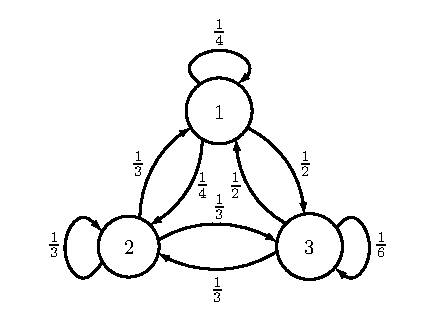
\includegraphics[width=\textwidth]{markov2}
\caption{Transition diagram}
\label{fig:markov2}
\end{figure}

\begin{enumerate}
\item Find the transition matrix.
\item If the Markov process is in state 1 initially, find the probability that it is in state 2 after two transitions.
\item Find the stable fixed point if it exists.
\end{enumerate}
\label{prob:markov_stablept}
\end{problem}
\end{comment}